\documentclass{article}
\usepackage[T2A,T1]{fontenc}
\usepackage[utf8]{inputenc}
\usepackage[russian]{babel}

\usepackage{amsmath}
\usepackage{graphicx}
\graphicspath{{images/}}
\usepackage{listings}
\usepackage[font=small,labelfont=bf]{caption}
\usepackage{csvsimple}
\usepackage{adjustbox}

\title{Параллельное программирование\\Лабораторная работа №1}
\author{ИИКС ИБ\\Б19-505\\Голигузов Алексей}
\date{Сентябрь 2021}

\begin{document}

\maketitle
\newpage
\tableofcontents

\newpage
\section{Рабочая среда}
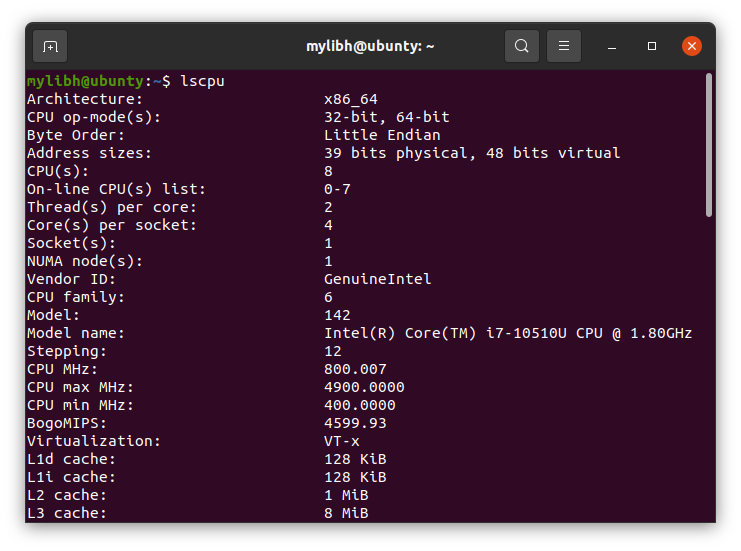
\includegraphics[width=\textwidth]{lscpu.png}
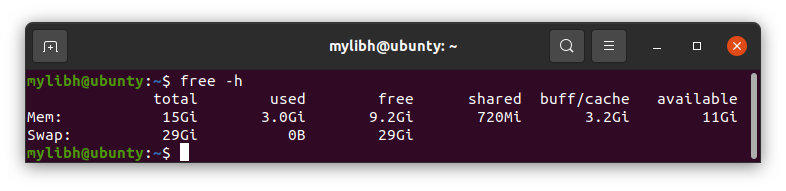
\includegraphics[width=\textwidth]{ram.png}
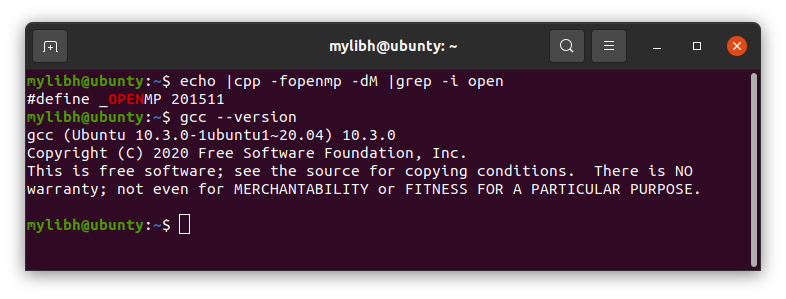
\includegraphics[width=\textwidth]{openmpgcc.png}
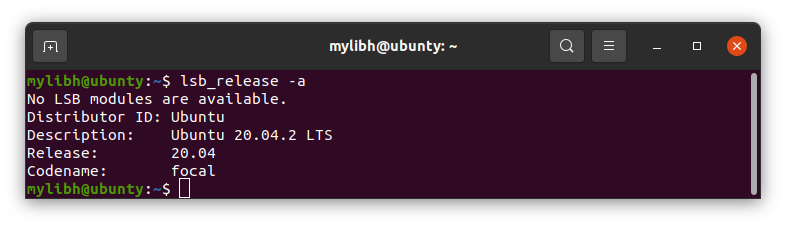
\includegraphics[width=\textwidth]{lsb.png}

\newpage
\section{Анализ}
Алгоритм работает за $O\left(\frac{n}{N}\right)$, где $n$ - кол-во данных, $N$ - кол-во потоков.
\begin{verbatim}
#pragma omp parallel for num_threads(threads_num) reduction(max: max)
\end{verbatim}
Распараллеливаем цикл на $threads\_num$ потоков, в конце собираем в $max$
локальные max со всех потоков.

\newpage
\section{Графики}
\begin{minipage}{\linewidth}
    \includegraphics[width=\linewidth]{time.png}
    \captionof{figure}{Время}
\end{minipage}
\begin{minipage}{0.48\linewidth}
    \includegraphics[width=\linewidth]{accel.png}
    \captionof{figure}{Ускорение}
\end{minipage}
\hfill
\begin{minipage}{0.49\linewidth}
    \includegraphics[width=\linewidth]{eff.png}
    \captionof{figure}{Эффективность}
\end{minipage}

\newpage
\section{Заключение}
\captionof*{figure}{Время}
\begin{minipage}{0.48\linewidth}
    \includegraphics[width=\linewidth]{time.png}
    \captionof{figure}{Разные}
\end{minipage}
\hfill
\begin{minipage}{0.49\linewidth}
    \includegraphics[width=\linewidth]{time_same.png}
    \captionof{figure}{Одинаковые}
\end{minipage}

\captionof*{figure}{Ускорение}
\begin{minipage}{0.48\linewidth}
    \includegraphics[width=\linewidth]{accel.png}
    \captionof{figure}{Разные}
\end{minipage}
\hfill
\begin{minipage}{0.49\linewidth}
    \includegraphics[width=\linewidth]{accel_same.png}
    \captionof{figure}{Одинаковые}
\end{minipage}
\captionof*{figure}{Эффективность}
\begin{minipage}{0.48\linewidth}
    \includegraphics[width=\linewidth]{eff.png}
    \captionof{figure}{Разные}
\end{minipage}
\hfill
\begin{minipage}{0.49\linewidth}
    \includegraphics[width=\linewidth]{eff_same.png}
    \captionof{figure}{Одинаковые}
\end{minipage}

\newpage
\section{Приложение 1}
\lstinputlisting[language=C]{src/lab1.c}

\newpage
\section{Приложение 1а}
\lstinputlisting[language=Python]{src/script.py}

\newpage
\section{Приложение 1б}
\lstinputlisting[language=bash]{src/build.sh}

\newpage
\section{Приложение 2}
\captionof{table}{Разные} 
\begin{adjustbox}{width=\linewidth}
    \begin{tabular}{|c|c|c|c|c|c|c|c|c|c|c|c|}
        \hline
        \bfseries Threads & \bfseries Avg&1&2&3&4&5&6&7&8&9&10
        \csvreader[head to column names]{src/data.csv}{}{\\\hline\csvlinetotablerow}
        \\\hline
    \end{tabular}
\end{adjustbox}

\captionof{table}{Одинаковые}
\begin{adjustbox}{width=\linewidth}
    \begin{tabular}{|c|c|c|c|c|c|c|c|c|c|c|c|}
        \hline
        \bfseries Threads & \bfseries Avg&1&2&3&4&5&6&7&8&9&10
        \csvreader[head to column names]{src/data_same.csv}{}{\\\hline\csvlinetotablerow}
        \\\hline
    \end{tabular}
\end{adjustbox}

\end{document}